\documentclass[conference]{IEEEtran}
\usepackage{paper}

% palette (Paul Tol's vibrant set, colour-blind safe): one hue per device,
% and green / red / blue for the decoding outcome
\definecolor{irA}{HTML}{0077BB}
\definecolor{irB}{HTML}{EE7733}
\definecolor{irC}{HTML}{AA3377}
\definecolor{irD}{HTML}{009988}
\definecolor{irOk}{HTML}{228833}
\definecolor{irSic}{HTML}{0077BB}
\definecolor{irLost}{HTML}{CC3311}
\DeclareRobustCommand{\figIrsa}{%
\begin{figure}[t]
  \centering
  \begin{tikzpicture}[
      font=\footnotesize, x=0.8cm, y=0.85cm, >=stealth,
      slot/.style={draw=gray!50, minimum width=0.8cm, minimum height=0.4cm, inner sep=0pt},
      rep/.style={draw, rounded corners=1.5pt, minimum width=0.62cm, minimum height=0.27cm, inner sep=0pt, font=\bfseries, text=white},
      lbl/.style={anchor=east, inner sep=2pt},
      sic/.style={->, thick, dashed, irSic},
    ]
    % one row per device, one column per slot: a replica is a coloured box
    \foreach \k/\col in {1/irA, 2/irB, 3/irC, 4/irD} {
      \node[lbl, text=\col] at (0.45, {2.5-0.5*\k}) {\k};
      \foreach \s in {1,...,5} { \node[slot] at (\s, {2.5-0.5*\k}) {}; }
    }
    \foreach \s in {1,...,5} { \node[text=gray!40!black, anchor=south, inner sep=1pt] at (\s, 2.23) {\s}; }
    % axes: time slots to the right, devices downward
    \draw[->, gray!40!black] (0.5, 2.62) -- node[above, inner sep=1pt] {time slot} (5.5, 2.62);
    \draw[->, gray!40!black] (0.05, 2.3) -- (0.05, 0.2);
    \node[rotate=90, anchor=south, inner sep=1pt] at (-0.12, 1.25) {device};
    \node[rep, fill=irA] (a1) at (1, 2.0) {1};  \node[rep, fill=irA] (a2) at (3, 2.0) {1};
    \node[rep, fill=irB] (b1) at (2, 1.5) {2};  \node[rep, fill=irB] (b2) at (3, 1.5) {2};
    \node[rep, fill=irC] at (4, 1.0) {3};  \node[rep, fill=irC] at (5, 1.0) {3};
    \node[rep, fill=irD] at (4, 0.5) {4};  \node[rep, fill=irD] at (5, 0.5) {4};
    % decoded singletons cancel their other replica along the row
    \draw[sic] (a1.east) -- (a2.west);
    \draw[sic] (b1.east) -- (b2.west);
    % the outcome per slot
    \node[text=irOk] at (1, 0.05) {\faCheck};
    \node[text=irOk] at (2, 0.05) {\faCheck};
    \node[text=irSic] at (3, 0.05) {\faCheck\,\textbf{SIC}};
    \node[text=irLost] at (4, 0.05) {\faTimes};
    \node[text=irLost] at (5, 0.05) {\faTimes};
    % legend, in the space right of the frame
    \node[anchor=west, align=left, inner sep=0pt] at (5.65, 1.2) {%
      \textcolor{irOk}{\faCheck} singleton\\[3pt]
      \textcolor{irSic}{\faCheck\,\textbf{SIC}}\\[3pt]
      \textcolor{irLost}{\faTimes} collision};
  \end{tikzpicture}
  \caption{An IRSA frame of $M = 5$ slots with four packets of $L = 2$ replicas.}
  \label{fig:irsa}
\end{figure}%
}

\usepackage{fontawesome5}
\usetikzlibrary{fit,backgrounds,positioning}
\colorlet{ovGreen}{green!45!black}
\colorlet{ovBlue}{blue!60!black}
\colorlet{ovOrange}{orange!85!black}
\colorlet{ovRed}{red!75!black}
\DeclareRobustCommand{\figSystemModel}{%
\begin{figure}[t]
  \centering
  \resizebox{\linewidth}{!}{%
  \begin{tikzpicture}[
      font=\scriptsize,
      >=stealth,
      box/.style={draw, rounded corners=2pt, align=center, inner sep=2pt, fill=white},
      panel/.style={draw, rounded corners=4pt, thick},
      tag/.style={draw, rounded corners=5pt, font=\tiny\bfseries, inner sep=1.5pt, text=white},
      rep/.style={draw, minimum width=0.17cm, minimum height=0.17cm, inner sep=0pt, font=\tiny},
      arr/.style={->, thick},
    ]

    % Real-world and synthetic traces replayed as ground-truth sources
    \node[panel, draw=gray!70, fill=gray!6, minimum width=8.8cm, minimum height=1.12cm] (data) at (4.4, 5.55) {};
    \node[tag, fill=gray!70!black, anchor=west] at ([xshift=4pt]data.north west) {Real-world and synthetic traces replayed as sources $X_k(n)$};
    \foreach \x/\icon/\name/\info [count=\i] in {
        1.1/\faThermometerHalf/Berkeley/232 sensors,
        3.3/\faBuilding/BTS/1633 sensors,
        5.5/\faIndustry/SINDIT/38 sensors,
        7.7/\faFlask/Synthetic/90 sensors} {
      \node[box, minimum width=2.1cm, minimum height=0.72cm] (ds\i) at (\x, 5.47) {};
      \node[anchor=north west, inner sep=1pt] at ([xshift=1pt, yshift=-1pt]ds\i.north west) {\icon~\texttt{\name}};
      \node[anchor=south west, inner sep=1pt, font=\tiny, text=gray!30!black] at ([xshift=1pt, yshift=0.5pt]ds\i.south west) {\info};
    }
    % Sparklines, bottom right of each box: smooth (Berkeley), fast-varying (BTS),
    % piecewise constant (SINDIT), slow drift with a burst (Synthetic)
    \draw[ovBlue, thick] plot[domain=0:0.75, samples=25, smooth] ({1.4+\x}, {5.3+0.07*sin(480*\x)});
    \draw[ovBlue, thick] (3.6,5.28) -- (3.66,5.38) -- (3.73,5.24) -- (3.8,5.36) -- (3.87,5.26) -- (3.94,5.4) -- (4.01,5.24) -- (4.08,5.35) -- (4.15,5.27) -- (4.22,5.38) -- (4.29,5.25);
    \draw[ovBlue, thick] (5.8,5.25) -- (6.0,5.25) -- (6.0,5.4) -- (6.3,5.4) -- (6.3,5.23) -- (6.55,5.23);
    \draw[ovBlue, thick] (8.0,5.25) -- (8.3,5.3) -- (8.38,5.42) -- (8.46,5.27) -- (8.75,5.33);

    % IoT device k: event trigger, proactive retransmission, background
    \node[box, draw=ovOrange, fill=orange!12, text width=3.45cm] (trig) at (1.875, 4.3)
      {\textbf{Event trigger}: transmit if\\$|X_k(n) - \text{record}| \ge \epsilon$};
    \node[box, draw=ovRed, fill=red!8, text width=3.45cm, below=3pt of trig] (rep)
      {\textbf{Proactive retransmission}:\\repeat w.p.\ $q$, up to $n_r$ times};
    \node[box, draw=ovBlue, fill=blue!8, text width=3.45cm, below=3pt of rep] (supp)
      {\textbf{Background}: transmit w.p.\ $x_{\mathrm{bg}}$};
    \begin{scope}[on background layer]
      \node[panel, draw=ovGreen, fill=green!6, fit=(trig)(rep)(supp), inner xsep=4pt, inner ysep=4pt,
            yshift=2pt, minimum height=0pt] (dev) {};
    \end{scope}
    \node[tag, fill=ovGreen, anchor=west] at ([xshift=4pt]dev.north west) {\faMicrochip~Stateless IoT device $k$};

    % IRSA frame with replicas, SIC and destructive collisions
    \node[font=\scriptsize\bfseries, anchor=south] at (5.3, 4.48) {IRSA frame, $M$ slots};
    \foreach \s in {0,...,4} {
      \draw[thick, fill=white] ({4.15+0.46*\s}, 3.55) rectangle ({4.61+0.46*\s}, 4.45);
    }
    \node[rep, fill=irA!55] at (4.38, 4) {1};
    \node[rep, fill=irB!60] at (4.84, 4) {2};
    \node[rep, fill=irA!55] at (5.3, 4.15) {1};
    \node[rep, fill=irB!60] at (5.3, 3.85) {2};
    \node[rep, fill=irC!50] at (5.76, 4.15) {3};
    \node[rep, fill=irD!50] at (5.76, 3.85) {4};
    \node[rep, fill=irC!50] at (6.22, 4.15) {3};
    \node[rep, fill=irD!50] at (6.22, 3.85) {4};
    \node[font=\tiny, text=ovGreen] at (4.38, 3.4) {\faCheck};
    \node[font=\tiny, text=ovGreen] at (4.84, 3.4) {\faCheck};
    \node[font=\tiny, text=ovGreen] at (5.3, 3.4) {SIC};
    \node[font=\tiny, text=ovRed] at (5.76, 3.4) {\faTimes};
    \node[font=\tiny, text=ovRed] at (6.22, 3.4) {\faTimes};
    \node[font=\tiny\bfseries, text=ovRed] at (5.99, 3.18) {lost, no ACK};
    \draw[arr] (trig.east) -- (4.15, 4.25);
    \draw[arr] (rep.east) -- (4.15, 3.8);

    % Base station, right-aligned with the panels so it clears the frame
    \node[panel, draw=ovBlue, fill=blue!5, text width=1.75cm, align=center, anchor=east] (bs) at (8.8, 4)
      {{\large\faBroadcastTower}\\[1pt]\textbf{Base station}\\SIC decoder,\\estimates $\hat{X}_k(n)$};
    \draw[arr] (6.45, 4) -- (bs.west);

    % The per-round schedule assignment is the only downlink signal
    \draw[arr, dashed, ovBlue] (bs.south) |- (supp.east);
    \node[font=\tiny, text=ovBlue, anchor=north, align=center] at (6.2, 2.82)
      {per round: schedule $\theta = (q, n_r, x_{\mathrm{bg}})$ per device,\\assigned via \tool (6 bits/device)};

    % AoII trajectory: a collided update stays stale until a retransmission is decoded
    \node[panel, draw=ovRed, fill=red!3, minimum width=8.8cm, minimum height=2.0cm] (aoii) at (4.4, 0.95) {};
    \node[tag, fill=ovRed, anchor=west] at ([xshift=4pt]aoii.north west) {Prolonged error periods and proactive retransmission};
    \draw[->, gray!60!black] (0.3, 0.3) -- (5.35, 0.3) node[below left, font=\tiny, inner sep=1pt] {slot $n$};
    \draw[->, gray!60!black] (0.3, 0.3) -- (0.3, 1.7) node[right, font=\tiny] {AoII $\Omega_k(n)$};
    \draw[ovRed, very thick, dashed] (1.0, 0.3) -- (5.1, 1.55) node[above left=1pt and 0pt, font=\tiny\bfseries] {\textsc{Reactive}};
    \draw[ovGreen, very thick] (0.3, 0.3) -- (1.0, 0.3) -- (2.7, 0.82) -- (2.7, 0.3) -- (5.2, 0.3) node[above left=0.5pt and 0pt, font=\tiny\bfseries] {\tool};
    \node[font=\tiny, text=ovRed] at (1.0, 0.42) {\faTimes};
    \node[font=\tiny, align=left, anchor=west] at (0.4, 1.3) {event trigger fires,\\update collides};
    \draw[gray, thin] (1.0, 0.52) -- (1.0, 1.08);
    \node[font=\tiny, text=ovGreen, align=left, anchor=south west] at (2.75, 0.32) {repeat\\decoded \faCheck};
    \node[font=\tiny, text=ovRed, align=left, anchor=north west] at (3.75, 1.05) {persistent error state:\\trigger remains silent};

    % Key findings
    \node[box, draw=ovRed, fill=red!10, text width=3.05cm, align=left, anchor=north west] (find1) at (5.55, 1.72)
      {\textcolor{ovRed}{\textbf{Local-record rules}}: $10^2\text{--}10^6\times$ higher AoII};
    \node[box, draw=ovGreen, fill=green!12, text width=3.05cm, align=left, below=4pt of find1] (find2)
      {\textcolor{ovGreen}{\textbf{\tool}}: 7\%--43\% higher reward at lowest load};
  \end{tikzpicture}%
  }
  \caption{System overview of \tool: stateless sensors follow an event trigger with proactive retransmissions and a background rate over a feedback-free IRSA uplink, while the base station optimizes the retransmission schedule $\theta$ via multiple-play Thompson sampling.}
  \label{fig:overview-arch}
\end{figure}%
}

\newcommand{\maintable}{%
  \begin{table}[t]
    \centering
    \caption{Steady-state AoII per policy, sorted from worst to best (mean $\pm$ standard deviation over ten seeds on the final 1000 slots; best in bold, $\dagger$: differs from the runner-up at $p < 0.01 $, Welch's $t$-test); last row: reward gain of \tool over the best baseline, $*$: significant at the Bonferroni level.}
    \label{tab:main}
    \setlength{\tabcolsep}{1pt}\scriptsize
    \begin{tabular*}{\columnwidth}{@{\extracolsep{\fill}}lrrrr@{}}
      \toprule
      \textbf{Policy} & \texttt{Synthetic} & \texttt{Berkeley} & \texttt{BTS} & \texttt{SINDIT} \\
      \midrule
      \textsc{Reactive} & $126{\pm}68$ & $241{\pm}127$ & $133{\pm}41$ & $1613{\pm}668$ \\
      \textsc{Threshold} & $3.1{\pm}2.3$ & $93{\pm}206$ & $69{\pm}69$ & $744{\pm}805$ \\
      \textsc{Hybrid} & $11{\pm}6$ & $0.498{\pm}0.264$ & $13{\pm}2$ & $0.0024{\pm}0.0035$ \\
      \textsc{VHCT} & $0.141{\pm}0.067$ & $0.046{\pm}0.016$ & $0.494{\pm}0.176$ & $0.0011{\pm}0.0018$ \\
      \textsc{Throughput} & $0.129{\pm}0.021$ & $0.040{\pm}0.007$ & $0.502{\pm}0.093$ & $0.0010{\pm}0.0009$ \\
      \tool (ours) & $\mathbf{0.048{\pm}0.028}$$^{\dagger}$ & $0.057{\pm}0.071$ & $\mathbf{0.277{\pm}0.206}$ & $0.0015{\pm}0.0031$ \\
      \textsc{UCB} & $0.121{\pm}0.050$ & $\mathbf{0.034{\pm}0.012}$ & $0.676{\pm}0.457$ & $\mathbf{0.0003{\pm}0.0003}$ \\
      \midrule
      \textit{reward gain} & +43\%$^{*}$ & +8\% & +38\% & +7\% \\
      \bottomrule
    \end{tabular*}
  \end{table}%
}

\newcommand{\hybridsupp}{$0.0023$, $0.0014$, and $0.0042$ on Berkeley, BTS, and SINDIT ($\hat p_E = 0.045$, $0.064$, and $0.008$)}
\newcommand{\robusttable}{%
  \begin{table}[t]
    \centering
    \caption{Sensitivity Across Operational Settings}
    \label{tab:robust}
    \setlength{\tabcolsep}{3.5pt}\scriptsize
    \begin{tabular*}{\columnwidth}{@{\extracolsep{\fill}}lrrr@{}}
      \toprule
      \textbf{Setting} & \textbf{Berkeley} & \textbf{BTS} & \textbf{SINDIT} \\
      \midrule
      Reference          & $1731\times$ / 0.86 & $53\times$ / 1.06 & $10^{5.7}\times$ / 0.56 \\
      Causal scaling     & $246\times$ / 1.65  & $23\times$ / 1.32 & $10^{5.2}\times$ / 0.57 \\
      $\epsilon = 0.005$ & $13\times$ / 0.83   & $1\times$ / 1.00  & $97\times$ / 0.63 \\
      $\epsilon = 0.02$  & $15\times$ / 0.57   & $1\times$ / 1.35  & $10^{4.0}\times$ / 0.47 \\
      $\alpha = 0.5$     & $22\times$ / 0.72   & $1\times$ / 0.87  & $356\times$ / 0.46 \\
      $\alpha = 2$       & $17\times$ / 0.83   & $1\times$ / 1.35  & $411\times$ / 0.41 \\
      $K = 20$           & $80\times$ / 0.68   & $483\times$ / 0.47 & $10^{6.4}\times$ / 0.39 \\
      $K = 40$           & $2566\times$ / 0.54 & $48\times$ / 2.33 & $10^{6.3}\times$ / 0.52 \\
      $L = 3$            & $2499\times$ / 0.89 & $62\times$ / 1.32 & $226\times$ / 0.52 \\
      Later time block   & $7929\times$ / 0.55 & --                & $10^{9.2}\times$ / 0.42 \\
      \bottomrule
    \end{tabular*}
  \end{table}%
}


\begin{document}

\title{An AoII Minimization Policy for IoT Sensor Traffic}

\author{
  \IEEEauthorblockN{Thanh Le\IEEEauthorrefmark{1}, Riccardo Cin\`a\IEEEauthorrefmark{2}, Hong-Linh Truong\IEEEauthorrefmark{3}, and Yusheng Ji\IEEEauthorrefmark{4}}
  \IEEEauthorblockA{\IEEEauthorrefmark{1}National Institute of Information and Communications Technology (NICT), Japan}
  \IEEEauthorblockA{\IEEEauthorrefmark{2}KTH Royal Institute of Technology, Sweden, \IEEEauthorrefmark{3}Aalto University, Finland}
  \IEEEauthorblockA{\IEEEauthorrefmark{4}National Institute of Informatics (NII) and The Graduate University for Advanced Studies (SOKENDAI), Japan}
}

\maketitle

\begin{abstract}
  Remote IoT sensors transmit sporadic updates to keep a base station informed of monitored physical processes.
  Age of incorrect information quantifies estimation quality at the receiver by penalizing both staleness and error magnitude.
  To support massive device populations, grant-free access omits per-packet acknowledgements, which breaks state-dependent sampling because an undetected collision leaves a sensor silent during subsequent quiet periods while the receiver estimate remains stale.
  To overcome these prolonged error periods, we instantiate \tool, a sampling framework for feedback-free grant-free uplinks.
  Under \tool, each sensor follows an event trigger with proactive retransmissions spread over subsequent slots, followed by a low background rate.
  The base station learns the retransmission schedule via multiple-play Thompson sampling from delayed batch feedback, keeping sensors stateless without local learning overhead.
  Evaluations across real-world and synthetic traces show that \tool improves reward by 7\%--43\% over the best baselines at the lowest channel load, maintains its performance across more than 200 sensors, and keeps its ranking over software-defined radios on the low-load trace, where physical receiver impairments penalize channel usage.
\end{abstract}

\begin{IEEEkeywords}
  Age of incorrect information, grant-free access, Internet of Things, multi-armed bandits
\end{IEEEkeywords}

\section{Introduction}
\label{sec:intro}

  Low-power Internet of Things (IoT) sensors in environmental monitoring, smart grids, and industrial digital twins generate sporadic telemetry over shared wireless uplinks~\cite{truong2022haivan,nguyen2024security}.
  For anomaly tracking and remote estimation, conventional freshness metrics that track only time since the last reception treat all packets equally regardless of how much the physical process has changed.
  Age of incorrect information (AoII), defined as the product of error magnitude and the duration for which the receiver's estimate has remained inaccurate, jointly penalizes staleness and value discrepancy~\cite{maatouk2022age}.
  Because constant transmission depletes batteries and congests shared radio resources, each sensor needs a policy that transmits selectively when updates meaningfully reduce AoII.

  \figSystemModel

  In massive machine-type communication (mMTC), coordinating individual transmissions or returning per-packet acknowledgements (ACKs) incurs prohibitive signaling overhead.
  Grant-free protocols such as irregular repetition slotted ALOHA (IRSA) eliminate handshake overhead by letting devices transmit packet replicas across frame slots resolved via successive interference cancellation (SIC) at the base station~\cite{munari2021modern}.
  However, operating without per-packet ACKs poses a fundamental challenge for state-dependent sampling.
  Existing AoII policies assume known Markov source dynamics and immediate ACKs~\cite{maatouk2022age,tong2023semantic,nayak2023decentralized}, or analyze feedback-free access on synthetic traffic models~\cite{munari2024monitoring,mubarak2026threshold}.
  When a device updates its local record upon transmitting without knowing whether the packet survived contention, an unacknowledged collision leaves the base station with a stale estimate.
  If the physical signal subsequently remains steady, the device remains silent while the base station stays in error indefinitely, inducing a persistent error state at the receiver.

  We instantiate \tool{} (\emph{\underline{M}ultiple-\underline{P}lay \underline{G}aussian \underline{T}hompson \underline{S}ampling}, \autoref{fig:overview-arch}), a lightweight sampling framework for feedback-free IRSA uplinks, alongside an end-to-end benchmark across three IoT sensor datasets~\cite{bodik2004intel,truong2022haivan,nguyen2024security}.
  \tool decouples local transmission from global schedule optimization.
  On the device side, each sensor follows an event trigger with proactive retransmission, sending repeated copies of its record spread over subsequent slots to clear collided updates without correlated re-collisions.
  On the base-station side, the network optimizes the retransmission schedule (repeat rate, repeat count, and background rate) as a multi-armed bandit via multiple-play Thompson sampling with a robust posterior scale.
  By assigning candidate schedules across all $K$ devices concurrently, the network converges rapidly from delayed round feedback while keeping the IoT sensors entirely stateless.

  The main contributions of this paper are as follows:
  \begin{itemize}
    \item An end-to-end benchmark coupling three IoT datasets (\texttt{Berkeley}, \texttt{BTS}, and \texttt{SINDIT}) and a \texttt{Synthetic} trace with controlled error periods, bursts, drift, and a regime change with a feedback-free IRSA uplink across disjoint sensor populations, causal normalization, operational variations, and 30 to 240 sensors.
    \item An empirical characterization showing that local-record policies (\textsc{Reactive} and \textsc{Threshold}~\cite{nayak2023decentralized,mubarak2026threshold}) degrade by up to six orders of magnitude in mean AoII as collided updates persist unrepaired during quiet periods.
    \item The \tool policy, which attains the highest reward across all four traces (gains of 7\%--43\% over the best baseline) at the lowest channel load among all policies that prevent persistent error states, and maintains its performance across more than 200~sensors.
    \item Component ablations and radio experiments on ADALM-Pluto hardware confirming that proactive retransmissions drive primary gains and that physical receiver impairments penalize channel usage, so the ranking holds on the low-load trace.
  \end{itemize}

\section{System Model}
\label{sec:system}

\subsection{Network Architecture and Grant-Free Access}
\label{sec:arch}
  We consider the grant-free monitoring network in \autoref{fig:overview-arch}, where $K$ synchronized IoT devices share a frame of $M$ uplink slots under IRSA without per-packet ACKs~\cite{munari2021modern}.
  Time is slotted with index $n \in \{1, \dots, N\}$ within each learning round $t \in \{1, \dots, T\}$.
  When a device transmits, it sends an average of $L < M$ packet replicas across randomly chosen slots of the frame.
  At the base station, an iterative SIC decoder resolves singleton slots containing one replica, cancels all other replicas of decoded packets across the frame, and repeats until no singletons remain; unresolved colliding packets are dropped, as \autoref{fig:irsa} illustrates.

  Within each slot $n$, operations follow a fixed sequence:
  (i) source $k$ takes its current value $X_k(n)$;
  (ii) device $k$ compares $X_k(n)$ against its local record of the last sent value;
  (iii) device $k$ decides whether to transmit under its policy;
  (iv) the base station decodes the frame and updates its estimate $\hat{X}_k(n)$ from decoded packets; and
  (v) lacking per-packet ACKs, device $k$ updates its local record to the sent value regardless of decoding outcome.
  The sole downlink signaling is a broadcast at the end of each round of $N$ slots.
  For the learned-supplement baselines, it is a delayed batch feedback reporting the round-average AoII (16-bit fixed-point) and decoded packet count (7 bits) per device (23 bits per device per round).
  For \tool, the broadcast consists solely of the assigned arm index for the next round (6 bits per device per round).
  Crucially, neither feedback identifies which slot collided, so devices cannot infer or repair stale local records from it.

\subsection{Age of Incorrect Information Metric}
\label{sec:metric}
  To capture both staleness and error magnitude at the base station, we adopt the distance-weighted AoII metric~\cite{maatouk2022age}.
  For device $k$ at slot $n$, the instantaneous AoII is defined as
  \begin{equation}
    \Omega_k(n) = \delta_k(n)\,(n - S_k(n)),
    \label{eq:aoii}
  \end{equation}
  where $\delta_k(n) := |X_k(n) - \hat{X}_k(n)|\,\mathbbm{1}\{|X_k(n) - \hat{X}_k(n)| \ge \epsilon\}$ weights estimation errors exceeding a tolerance $\epsilon > 0$, and $S_k(n)$ is the last slot at which the receiver's estimate became erroneous.
  Intuitively, $\Omega_k(n)$ stays zero while $\hat{X}_k(n)$ lies within $\epsilon$ of $X_k(n)$, and grows linearly with error duration scaled by the discrepancy once an inaccurate estimate occurs.

  \figIrsa

\subsection{Problem Formulation}
\label{sec:problem}
  Let $u_k(t) \in [0,1]$ denote the fraction of the $N$ slots in round $t$ in which device $k$ initiates a transmission, each occupying $L$ slot replicas on average.
  At the start of round $t$, device $k$ chooses a randomized transmission probability $x_k \in [0, \overline{x}]$ to minimize its cumulative AoII and transmission cost:
  \begin{equation}
    \underset{x_k \in [0, \overline{x}]}{\text{minimize}} \;
    \sum_{t=1}^{T} \Big[ \frac{1}{N}\sum_{n=1}^{N} \Omega_k(n) + \alpha\, u_k(t) \Big],
    \label{eq:problem}
  \end{equation}
  where $\alpha > 0$ weights transmission cost against AoII and $\overline{x}$ is the symmetric per-device probability that maximizes IRSA throughput when adopted by all devices~\cite{munari2021modern}.
  Aggregate contention is measured by the \emph{offered load} $G = \frac{1}{M}\sum_{k=1}^K u_k(t)$, representing the mean number of transmissions started per IRSA slot; for $K = 30$, $M = 5$, and $\overline{x} = 0.55\,M/K \approx 0.092$, operating every device at $\overline{x}$ gives $G = 0.55$.

\section{Proposed AoII Minimization Policy}
\label{sec:propose}

\subsection{Prolonged Error Periods under Local Records}
\label{sec:desync}
  This section explains the failure mode the proposed policy is designed to address, so that each component can be understood as a direct response to it.
  Without acknowledgements, a device learns nothing about the fate of a packet, so local-record rules update the record of the last sent value as if the packet had arrived.
  When the packet collided, the record and the reading agree while the base station holds an outdated estimate, and the trigger stays silent until the source moves again.
  \autoref{fig:markov} abstracts this as a two-state chain: device $k$ leaves the correct state $C_k$ when a move (probability $p_E$ per slot) fires a trigger that is lost (probability $p_\ell$), and returns from the erroneous state $W_k$ at a recovery rate $r_k$ that collects every event that refreshes $\hat{X}_k$.
  With a sojourn in $W_k$ geometric of mean $1/r_k$ and a mean mismatch $\bar\delta_k$, the expected per-slot AoII is
  \begin{equation}
    \bar\Omega_k = \frac{\bar\delta_k\, p_E\, p_\ell}{r_k\,(p_E p_\ell + r_k)},
    \label{eq:aoii-model}
  \end{equation}
  since each sojourn accumulates $\bar\delta_k W(W+1)/2$ of AoII over $W$ slots.
  For a purely \textsc{Reactive} device, the only recovery event is the next move, $r_k = p_E(1-p_\ell)$, and~\eqref{eq:aoii-model} reduces to $\bar\delta_k p_\ell / [(1-p_\ell) p_E]$, the closed form of~\cite{munari2024monitoring}: the quieter the source, the longer the error period persists.
  Intuitively, the penalty of a lost trigger scales as $1/p_E^2$ while the transmission cost of an additional packet is constant, so quiet sources benefit most from dedicating channel usage to proactive~packet~retransmissions.

  \begin{figure}[t]
    \centering
    \begin{tikzpicture}[->, >=stealth', auto, semithick, node distance=2.6cm]
      \tikzstyle{every state}=[fill=white,draw=black,thick,text=black,scale=0.85]
      \node[state]    (A)                {$C_k$};
      \node[state]    (B)[right of=A]    {$W_k$};
      \path
      (A) edge[loop left]     node{\scriptsize $1 - p_E p_\ell$}    (A)
      (B) edge[loop right]    node{\scriptsize $1 - r_k$}    (B)
      (A) edge[bend left]     node{\scriptsize $p_E\, p_\ell$}    (B)
      (B) edge[bend left]     node{\scriptsize $r_k$, \eqref{eq:repair}}    (A);
    \end{tikzpicture}
    \caption{Two-state AoII chain of device $k$ between the correct state $C_k$ and the erroneous state $W_k$.}
    \label{fig:markov}
  \end{figure}

\subsection{Device Policy: Event Trigger and Proactive Retransmission}
\label{sec:device}
  The device side of \tool needs no learning and no per-device signalling beyond the schedule it is assigned.
  In slot $n$, device $k$ transmits when its reading differs from its local record by more than $\epsilon$ (the \emph{event trigger}), exactly as the local rules do.
  Because it cannot know whether that packet survived, it performs \emph{proactive retransmissions}: it re-sends the record with probability $q$ in every following slot until it has re-sent it $n_r$ times or the next trigger restarts the count, and with a \emph{background} probability $x_{\mathrm{bg}}$ after that, which bounds the error duration that survives all repeats.
  Writing $m_k(n)$ for the number of re-sends since the last trigger, the device's whole logic is a transmission probability that depends on this one counter,
  \begin{equation}
    \pi_\theta(m) = \begin{cases} q & m < n_r, \\ x_{\mathrm{bg}} & m \ge n_r, \end{cases}
    \qquad \theta = (q, n_r, x_{\mathrm{bg}}),
    \label{eq:schedule}
  \end{equation}
  applied whenever the trigger is silent; every transmission occupies $L$ replicas of the IRSA frame.
  We call $\theta$ the \emph{retransmission schedule}; \autoref{sec:learn} leaves its choice entirely to the base station.

  Two design choices follow from \autoref{sec:desync}.
  First, the repeats are conditioned on a trigger, so a quiet device incurs no channel usage, whereas a uniform random supplement~\cite{munari2024monitoring} charges every device the same rate and must stay small to keep the load within the IRSA budget; a lost trigger is then resolved only after $1/x$ slots on average.
  With repeats, a lost trigger is resolved after $1/q$ slots on average, and the probability that the trigger and all $n_r$ repeats are lost is $p_\ell^{\,n_r+1}$, so the recovery rate of \autoref{fig:markov} becomes
  \begin{equation}
    r_k = 1 - (1 - \pi_\theta(m_k) (1 - p_\ell))\,(1 - p_E (1 - p_\ell)),
    \label{eq:repair}
  \end{equation}
  which equals $q(1-p_\ell)$ to first order right after a trigger and decays to the background rate once the budget is spent.
  Second, the repeats are spread in time by the per-slot probability $q$ because triggers are correlated across devices: the sensors of one room warm up together and the actuators of one factory cell switch together, so the triggered packets that collided in a frame would collide again if every device repeated immediately in the next~frame.

\subsection{Base-Station Learning of the Retransmission Schedule}
\label{sec:learn}
  \begin{algorithm}[t]
    \caption{\tool Schedule Learning at the Base Station}
    \label{alg:mpgts}
    \footnotesize
    \begin{algorithmic}[1]
      \REQUIRE Candidate schedule grid $\Theta$, device population $K$, round length $N$.
      \STATE Initialize $n_0(\theta) \leftarrow 0$, $\hat\mu_0(\theta) \leftarrow +\infty$ ($\forall \theta \in \Theta$), $\mathcal{R} \leftarrow \emptyset$.
      \FOR{each round $t = 1, \dots, T$}
        \STATE $\hat\sigma_t \leftarrow 1.4826\,\mathrm{median}(|\mathcal{R} - \mathrm{median}(\mathcal{R})|)$ if $|\mathcal{R}| \ge 2$ else $1$.
        \FOR{each device $k = 1, \dots, K$}
          \STATE Sample $\tilde\mu_k(\theta) \sim \mathcal{N}(\hat\mu_{t-1}(\theta), \hat\sigma_t^2 / n_{t-1}(\theta))$ for all $\theta \in \Theta$.
          \STATE Assign $\theta_k(t) \leftarrow \arg\max_{\theta \in \Theta} \tilde\mu_k(\theta)$.
        \ENDFOR
        \STATE Broadcast indices $\{\theta_k(t)\}_{k=1}^K$; execute $N$ IRSA slots via~\eqref{eq:schedule}.
        \STATE Compute per-device rewards $r_k(t)$ via~\eqref{eq:reward} for $k = 1, \dots, K$.
        \FOR{each played schedule $\theta$ with $\mathcal{K}_\theta = \{k : \theta_k(t) = \theta\}$}
          \STATE Append within-arm residuals $\{r_k(t) - \bar r_\theta\}_{k \in \mathcal{K}_\theta}$ to $\mathcal{R}$.
          \STATE Update $n_t(\theta) \leftarrow n_{t-1}(\theta) + |\mathcal{K}_\theta|$ and running mean $\hat\mu_t(\theta)$.
        \ENDFOR
      \ENDFOR
    \end{algorithmic}
  \end{algorithm}

  The schedule trades lingering error periods in~\eqref{eq:repair} against transmission cost, and its optimal value depends on source dynamics; \autoref{sec:rq2} shows that no fixed schedule excels across all traces.
  We formulate schedule selection as a multi-armed bandit at the base station (\autoref{alg:mpgts}) over a discrete candidate grid $\Theta$ of schedules $\theta = (q, n_r, x_{\mathrm{bg}})$.
  At the end of each round of $N$ slots, the base station evaluates each device's round reward from~\eqref{eq:problem},
  \begin{equation}
    r_k(t) = - \frac{1}{N} \sum_{n=1}^{N} \big[\Omega_k(n) + \alpha\, a_k(n)\big],
    \label{eq:reward}
  \end{equation}
  where $a_k(n) \in \{0, 1\}$ marks a transmission, credits $r_k(t)$ to the played schedule $\theta_k(t)$, and broadcasts the next assignment.

  Two properties shape \autoref{alg:mpgts}.
  First, while an operational horizon may afford few rounds, every round yields $K$ device outcomes, enabling multiple-play Thompson sampling~\cite{thompson1933likelihood,agrawal2012analysis,komiyama2015optimal} (lines 4--7): while posteriors are wide, the $K$ devices explore distinct schedules concurrently; as posteriors sharpen, draws concentrate on a single schedule without a manual exploration constant.
  Second, per-device rewards exhibit a heavy-tailed reward distribution with outlier penalties from prolonged error periods (\autoref{sec:desync}) that would inflate the sample standard deviation.
  Line~3 therefore sets $\hat\sigma_t$ to $1.4826$ times the median absolute deviation of within-arm residuals (\autoref{sec:rq2} ablates this choice along with \textsc{UCB} and \textsc{VHCT}~\cite{li2021optimum} learners).

\subsection{Consistency of the Learned Schedule}
\label{sec:theory}
  This section states the property that justifies leaving the schedule to the base station: under stationary traffic the learner settles on the schedule with the best expected reward, and the device side keeps the AoII of every schedule with a background bounded.

  \begin{assumption}[Stationary traffic]
  \label{as:stationary}
  Over the horizon, every device moves with a fixed probability $p_E$ per slot and loses each packet with a fixed probability $p_\ell$, independently across rounds, so that the per-device rewards~\eqref{eq:reward} credited to a schedule $\theta$ are independent and identically distributed with a finite mean $\mu(\theta)$ and the robust scale $\hat\sigma_t$ stays bounded; the maximizer $\theta^\star$ of $\mu$ over the grid is unique; and every schedule is credited infinitely often.
  \end{assumption}
  The fixed $p_\ell$ abstracts the contention of the other devices as a mean field, as in~\cite{le2024mftts}, and the last clause holds for Thompson sampling because a Gaussian posterior sample gives every arm a positive probability in every round~\cite{agrawal2012analysis}.

  \begin{theorem}
  \label{thm:consistency}
  Under Assumption~\ref{as:stationary}, let $\hat\mu_t(\theta)$ be the posterior mean of schedule $\theta$ after $t$ rounds.
  \begin{enumerate}
    \item[(i)] For every $\theta$, $\hat\mu_t(\theta) \to \mu(\theta)$ almost surely, and almost surely $\theta^\star$ is the unique maximizer of $\hat\mu_t$ for all but finitely~many~rounds.
    \item[(ii)] The probability that a device is assigned a schedule other than $\theta^\star$ in round $t$ tends to zero.
    \item[(iii)] Under a schedule that transmits with probability at least $x = \min(q, x_{\mathrm{bg}}) > 0$ in every slot after a trigger, the mean AoII~\eqref{eq:aoii-model} is at most $\bar\delta_k p_E p_\ell / [x(1 - p_\ell)]^2$, and the \textup{\textsc{Reactive}} device's mean AoII, $\bar\delta_k p_\ell / [(1 - p_\ell) p_E]$, exceeds it by a factor of at least $x^2 (1 - p_\ell) / p_E^2$.
  \end{enumerate}
  \end{theorem}

  \begin{proof}[Proof sketch]
  (i) The rewards credited to $\theta$ form an i.i.d.\ sequence, and $\hat\mu_t(\theta)$ is its running mean along the number of credited device-rounds, which grows without bound, so the strong law of large numbers gives $\hat\mu_t(\theta) \to \mu(\theta)$ almost surely.
  With finitely many schedules and the gap $\Delta = \mu(\theta^\star) - \max_{\theta \neq \theta^\star} \mu(\theta) > 0$, every posterior mean is within $\Delta/2$ of its limit from some round on, and $\theta^\star$ is then the unique maximizer.
  (ii) A posterior sample is $\hat\mu_t(\theta) + \hat\sigma_t Z / \sqrt{n_t(\theta)}$ with $Z$ standard normal.
  The posterior mean converges in probability by (i), and the noise term vanishes in probability because $\hat\sigma_t$ is bounded, $n_t(\theta) \to \infty$, and Chebyshev's inequality bounds the tail of $Z$; a union bound over the schedules shows that every sample is within $\Delta/2$ of its mean with probability tending to one, which forces the sampled maximizer to be $\theta^\star$.
  (iii) The mean AoII~\eqref{eq:aoii-model} decreases in $r_k$ and is at most $\bar\delta_k p_E p_\ell / r_k^2$, and~\eqref{eq:repair} gives $r_k \ge x (1 - p_\ell)$ in every slot; the \textsc{Reactive} rate $r_k = p_E (1 - p_\ell)$ gives the closed form, and the ratio of the two is the stated factor.
  \end{proof}
  Intuitively, the only quantity to learn, $\theta^\star$, is a function of the traffic statistics that the base station observes for every device at once, so the devices need no learner; and the background of the device policy is what keeps the reward of every schedule finite, so that the posterior means the base station compares are averages of bounded penalties, whereas a schedule without background exposes them to the persistent error states of \autoref{sec:desync}.
  \autoref{fig:scaling} shows (ii) empirically as the share of devices on one schedule.

\section{Performance Evaluation}
\label{sec:result}

  \begin{figure}[t]
    \centering
    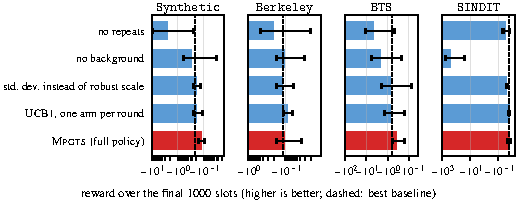
\includegraphics{figure/simulation/plot_ablation.pdf}
    \caption{Ablation of \tool per trace, sorted from worst (top) to best; red: full policy, dashed: best baseline of \autoref{tab:main}.}
    \label{fig:ablation}
  \end{figure}

  Our evaluation investigates the following research questions:
  \noindent\textbf{RQ1} (\autoref{sec:rq1}): How does \tool compare with local-record rules, fixed access rules, and learned supplements in AoII, load, and reward? \\
  \noindent\textbf{RQ2} (\autoref{sec:rq2}): What do proactive retransmissions, the background rate, and the placement of the learner each contribute? \\
  \noindent\textbf{RQ3} (\autoref{sec:rq3}): How do the gains hold under protocol variations and with more sensors? \\
  \noindent\textbf{RQ4} (\autoref{sec:rq4}): Does the policy ranking under idealized slot-occupancy decoding hold over software-defined radios?

\subsection{Experimental Setup}
\label{sec:setup}

\subsubsection{Traces and Preprocessing}
  To assess controlled traffic dynamics, we generate a \textbf{\texttt{Synthetic}} benchmark of 90 sensors combining quiet periods, random walks, drift, and correlated bursts, with an event-rate doubling at slot $10{,}000$.
  We further evaluate policies over three public IoT sensor datasets:
  \textbf{\texttt{Berkeley}}~\cite{bodik2004intel} (temperature, humidity, light, and voltage across 232 indoor sensors),
  \textbf{\texttt{BTS}}~\cite{truong2022haivan} (smart-building and environmental telemetry from 1633 sensors), and
  \textbf{\texttt{SINDIT}}~\cite{nguyen2024security} (actuator-driven industrial telemetry across 38 sensors).

  Each device replays one stream as ground truth $X_k(n)$, sampling the latest measurement at slot interval $\Delta$ (fixed to the median inter-event time: $35.2$~s on \texttt{Berkeley}, $18.0$~s on \texttt{BTS}, and $3.0$~s on \texttt{SINDIT}).
  Streams are normalized to $[0,1]$ by min--max scaling.
  Evaluation horizons span $T = 20{,}000$ slots on \texttt{Synthetic}, $T = 10{,}000$ on \texttt{Berkeley} and \texttt{SINDIT}, and $T = 3{,}000$ on \texttt{BTS}.
  The primary network comprises $K = 30$ sensors, with additional disjoint 30-sensor subsets evaluated in \autoref{sec:rq3}.

\subsubsection{Baselines and Channel Configuration}
  The default IRSA uplink operates with $K = 30$ devices over frames of $M = 5$ slots, $L = 2$ replicas, error tolerance $\epsilon = 0.01$, and cost weight $\alpha = 1$.
  We benchmark \tool against six baselines across three access paradigms:
  \begin{itemize}
    \item \emph{Local-record rules}: \textsc{Reactive}~\cite{munari2024monitoring} transmits solely upon an event trigger ($|X_k(n) - \hat{X}_k(n)| \ge \epsilon$); \textsc{Threshold}~\cite{nayak2023decentralized,mubarak2026threshold} transmits once a local AoII proxy crosses threshold $\tau$.
    \item \emph{Fixed random access}: \textsc{Throughput}~\cite{munari2024monitoring} transmits with fixed rate $\overline{x} = 0.55\,M/K \approx 0.092$; \textsc{Hybrid}~\cite{munari2024monitoring} augments the event trigger with a fixed supplement $x_h = 0.05\,(\overline{x} - \hat p_E)^+$.
    \item \emph{Learned supplements}: \textsc{UCB} (\textsc{Ucb1} over a candidate parameter grid) and \textsc{VHCT}~\cite{li2021optimum} (hierarchical bandit trees over the continuous space) adapt a per-device uniform supplement over $[0, \overline{x}]$ under round feedback.
  \end{itemize}
  \tool learns over a candidate grid $\Theta$ of $|\Theta| = 36$ schedules formed by $q \in \{0.02, 0.05, 0.1\}$, $n_r \in \{1, 3, 5\}$, and $x_{\mathrm{bg}} \in \{0, 0.002, 0.01, 0.03\}$, with round length $N = 25$ slots.

\subsubsection{Evaluation Protocol}
  Every simulated configuration is evaluated over ten random seeds varying IRSA slot selections and policy decisions, and every radio configuration over five, the budget of a single set of three radios.
  Differences between policies are tested with Welch's $t$-test on the per-seed values at level $0.01$, Bonferroni-corrected over the six baselines for the gain of \tool and uncorrected for the comparison of the two best policies.
  Performance metrics are averaged over the final 1000 slots of each run and reported as mean $\pm$ standard deviation.
  Every number below is produced by \texttt{make results} in the released code, which also writes \autoref{tab:main} and \autoref{fig:ablation}--\ref{fig:ota}.

\subsection{RQ1: Policy Comparison Across IoT Traces}
\label{sec:rq1}

  \autoref{tab:main} sorts the policies by their steady-state AoII.
  \tool attains the lowest AoII on \texttt{Synthetic} and \texttt{BTS}, 60\% and 44\% below the best baseline.
  On \texttt{Berkeley} and \texttt{SINDIT}, \textsc{UCB} reaches a lower AoII only by imposing $1.6\times$ and $3.7\times$ higher load ($G = 0.49$ and $0.34$ versus $0.30$ and $0.09$ for \tool); consequently, \tool secures the highest reward~\eqref{eq:problem} across all four traces, with gains of 43\%, 8\%, 38\%, and 7\% over the strongest baseline on \texttt{Synthetic}, \texttt{Berkeley}, \texttt{BTS}, and \texttt{SINDIT}.
  Under Welch's $t$-test on the per-seed rewards against that baseline, the gain is significant on \texttt{Synthetic} ($p = 2 \cdot 10^{-7}$, below the Bonferroni level of $0.01/6$), reaches $p = 0.007$ on \texttt{BTS}, and lies within the seed variation on \texttt{Berkeley} and \texttt{SINDIT} ($p = 0.70$ and $0.46$), where \tool matches the best baseline at a lower load.

  The local-record rules \textsc{Reactive} and \textsc{Threshold} incur $64\times$ to $10^{5.7}\times$ higher AoII than \tool due to persistent error states~(\autoref{sec:desync}): undetected collisions leave the base station in stale error until the source moves again~\cite{munari2024monitoring}, compounding quadratically on piecewise-constant traces like \texttt{SINDIT} where actuators remain static for prolonged intervals.
  The learned supplements avoid these states but settle near the centre of their rate domain and pay in load, whereas \tool tailors its schedule to trace dynamics: it adopts higher retransmission rates and moderate background probing on bursty \texttt{Synthetic} telemetry, $(q, n_r, x_{\mathrm{bg}}) = (0.080, 3.7, 0.008)$, while selecting extensive proactive repeats with virtually zero background rate on quiet \texttt{SINDIT} streams, $(0.039, 3.7, 0.0004)$.

\subsection{RQ2: Ablation of Schedule, Proactive Retransmission, and Learner}
\label{sec:rq2}

  \maintable

  \begin{figure}[t]
    \centering
    
\includegraphics{figure/simulation/plot_scaling_legend.pdf}\\[-2pt]
    \subfloat[Reward per policy]{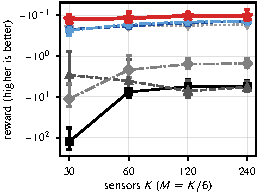
\includegraphics{figure/simulation/plot_scaling_reward.pdf}\label{fig:scaling-reward}}
    \hfill
    \subfloat[Rounds to consensus of \tool]{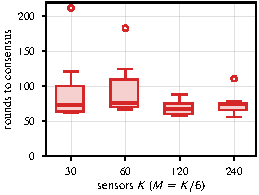
\includegraphics{figure/simulation/plot_scaling_consensus.pdf}\label{fig:scaling-consensus}}
    \caption{Scaling on \texttt{Synthetic} with $K$ sensors over $M = K/6$ slots (ten seeds): reward per policy, and the rounds until 80\% of the devices share one schedule.}
    \label{fig:scaling}
  \end{figure}

  \begin{figure}[b]
    \centering
    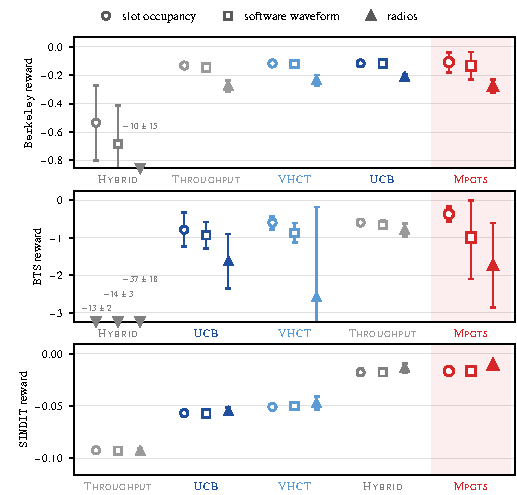
\includegraphics{figure/simulation/plot_ota.pdf}
    \caption{Reward per policy under slot-occupancy decoding, the software waveform, and the radios, sorted from worst to best; \textsc{Reactive} and \textsc{Threshold} lie below $-10$ on every channel and are omitted; off-scale values are marked at the axis edge with their mean $\pm$ standard deviation.}
    \label{fig:ota}
  \end{figure}

  \autoref{fig:ablation} removes or replaces one component of \tool at a time, and only the full policy beats the best baseline on all four traces.
  Proactive retransmission contributes most: eliminating repeats reduces the policy to a \textsc{Reactive} trigger with an unconditioned supplement, losing $20\times$ on \texttt{Synthetic} and $12\times$ on \texttt{BTS}.
  Without a background, a collided repeat leaves the device silent until its next trigger, driving reward on \texttt{SINDIT} down to $-272$.

  The learner components matter where rewards are heavy-tailed or rounds are scarce.
  Rare error-period penalties inflate conventional variance, artificially widening posterior intervals; substituting sample standard deviation for the robust scale $\hat\sigma_t$ incurs a $2.0\times$ penalty on \texttt{BTS}.
  Furthermore, single-play \textsc{Ucb1} degrades reward by 52\% on \texttt{BTS}, because sequentially testing 36 arms over 120 rounds starves the learner of per-arm observations.

\subsection{RQ3: Robustness and Scaling}
\label{sec:rq3}

  Across thirteen protocol variations per trace (evaluating causal scaling, frozen learning, sensitivity across $\epsilon$, $\alpha$, $K$, $L$, an alternate time block, and disjoint 30-stream partitions), \tool achieves first rank in 36 of 51 configurations and ranks within the top two in 42.
  Marginal drops occur primarily under tight round budgets on \texttt{BTS} and under causal scaling, where nonstationary drift beyond the calibration horizon penalizes exploration of arms with few repeats.

  \autoref{fig:scaling} examines scalability on \texttt{Synthetic} with $K \in \{30, 60, 120, 240\}$ devices over $M = K/6$ slots.
  Each device maintains only a single repeat counter and a 3-tuple schedule, while the base station draws $36K$ posterior samples and broadcasts $K$ six-bit arm indices per round.
  \tool maintains superior reward at all device densities, staying between $-0.102$ and $-0.126$.
  Crucially, the rounds until 80\% of the devices share one schedule do not grow with the sensor count: the median lies between 67 and 77 rounds at every $K$ (\autoref{fig:scaling-consensus}), because the $K$ attributed observations per round sharpen the posteriors in step with the number of devices they serve.

\subsection{RQ4: Over-the-Air Radio Evaluation}
\label{sec:rq4}

  We benchmark policies over an orthogonal frequency-division multiplexing (OFDM) waveform with waveform-level SIC, both in software simulation at $20$~dB SNR and over three ADALM-Pluto software-defined radios operating at $915$~MHz: one radio transmits for the device under test, a second emulates aggregate contention, and a third acts as base station.
  Hardware imperfections cut per-device delivery at four concurrent transmissions from $0.70$ under idealized slot occupancy down to $0.41$ over the radios.

  \autoref{fig:ota} shows that physical decoding penalizes channel usage.
  Over the radios, the delivery of \tool falls from $0.79$ to $0.47$ on \texttt{Berkeley} and from $0.67$ to $0.45$ on \texttt{BTS}, where its learned load is $0.49$ and $0.56$, and stays at $0.87$ on \texttt{SINDIT}, where the learned schedule transmits in 6\% of the slots.
  The simulated ranking therefore holds on \texttt{SINDIT}, where \tool remains first on all three channels ($-0.010$ against $-0.013$ for \textsc{Hybrid} over the radios), and reverses on the two high-load traces: on \texttt{Berkeley}, \textsc{UCB} ($-0.21$), \textsc{VHCT} ($-0.24$) and \textsc{Throughput} rank ahead of \tool ($-0.28$), and on \texttt{BTS} every learned policy falls behind \textsc{Throughput} ($-0.79$), with \tool at $-1.7$, where its load of $0.56$ costs delivery and one of five seeds collapses to $-3.7$ on the 120-round horizon, the risk of \autoref{sec:rq3}.
  The radios thus confirm the mechanism of \autoref{sec:desync} on hardware: the gains of \tool survive where it learns a low load, and short or busy traces call for the load-aware exploration left to future work.

\section{Related Work}
\label{sec:related}

  AoII-aware scheduling has been widely investigated under known source statistics and acknowledged links~\cite{maatouk2022age,bountrogiannis2024age,kriouile2023when,hong2024age,tong2023semantic}, but these approaches optimize thresholds, Whittle index policies, or NOMA allocations assuming per-packet ACKs or Markov transition matrices unavailable in grant-free uplinks.
  In random access channels, age of information has been analyzed under IRSA~\cite{munari2021modern,saha2021minimum} and feedback-free slotted ALOHA~\cite{munari2024monitoring,mubarak2026threshold,chiariotti2025distributed}, but existing studies rely on synthetic Markov sources under idealized collision models without physical waveform validation or schedule adaptation for nonstationary traffic.
  Learning-based massive access optimizes multi-agent reinforcement learning for resource selection~\cite{le2022tinyqmix} or mean-field Thompson sampling for power allocation~\cite{le2024mftts}, but requires per-device learners and targets access delay or transmit power rather than AoII.

\section{Conclusion}
\label{sec:conclusion}

  This paper demonstrated that mitigating unacknowledged collisions in grant-free random access requires proactive, localized retransmissions to prevent persistent error states.
  By coupling open-loop repetition with base-station multiple-play Thompson sampling, \tool adapts to diverse IoT dynamics without local device overhead.
  Over-the-air experiments confirm that physical SIC impairments penalize channel usage beyond idealized collision models, favoring policies that contain contention.
  Future work will explore scale normalization for nonstationary sensor drift and personalized schedule assignments.

\section*{Acknowledgement}

  The authors thank John C.S.\ Lui of The Chinese University of Hong Kong (CUHK) for his insightful discussions.
  This research is supported in part by JST ASPIRE~(JPMJAP2325).

\printbibliography
\end{document}
